\subsection{Transfer Learning}\label{sec:Transfer}
\par
Transfer learning is a well-known and often used strategy when it comes to the task at hand of this report, i.e. classification.  \textbf{\textit{Karthik E}}\autocite{e2021framework}s report suggests that high accuracy classification can be achieved when using transfer learning compared to both traditional machine learning used in a previous paper by \textbf{\textit{Karthik E}} and a baseline model using only the source domain model with no training. The basics of the transfer learning task is to retrieve learned features from an existing model with a specific domain. The retrieved features can then be mapped together with the target domain, in the case of this project together with the \hyperref[sec:DRE19]{Danish Real Estate Dataset}. \textbf{\textit{Pan Yang}} \autocite{PanYang2010} introduces a definition for transfer learning, from this definition it is possible to categorise the transfer learning task faced in this project. In the paper two different cases are described, the first case where the feature spaces of the domains are different, and the second case where the feature spaces are the same, but the marginal probability is different. In this project, the first case is the proper one to use. Both images and labels have been available in the completion of this project, and therefore the inductive transfer learning implementation is chosen.
\begin{figure}[H]
    \centering
    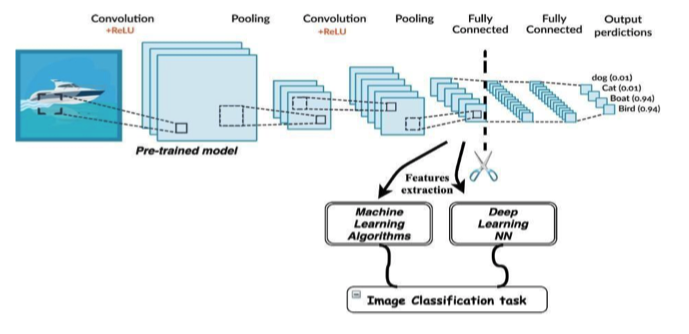
\includegraphics[width =\textwidth]{pictures/random/Transferlearning}
    \caption{Transfer Learning applied to a CNN.\\
    Image from: https://arxiv.org/pdf/2101.00793.pdf page. 10}
    \label{ref:TransferLearning}
\end{figure}
The figure above, \autoref{ref:TransferLearning}, show how the transfer learning task is applied to a convolutional neural network. The pre-trained classification layer is discarded, the features are extracted and another classification layer is trained on top of the pre trained model. The pre-trained model can distinguish between four different categories, dog, cat, boat and bird. In the transfer learning stage, it will be possible to create multiple completely new categories, for example: motor boat, sail boat, row boat, canoe and a raft. Because the pre trained network know how to represent a feature space of a boat, it might be possible to teach it how to distinguish between different kinds of boats.\par
As shown later it is possible to implement this technique to train two general-domain models, \hyperref[sec:resnet50]{Resnet50} and \hyperref[sec:effecientnet]{EffecientNetB0}, to accurately categories and represent the feature spaces of the rooms of the \hyperref[sec:DRE19]{Danish Real Estate} dataset.
% Most applications of machine learning methods rely on input originating from a domain with shared characteristics.
% This is often observed practical applications of machine learning; train a model to predict in a particular domain such as predicting whether an image is of a cat or a dog.
% This is referred to as the traditional supervised learning paradigm.
% Models developed within this paradigm can be proficient at solving the stated training objective, but fail to generalize to new information and require extensive retraining in order to perform with new data or classes.
% \newline
% Models trained to solve supervised learning objectives often exhibit similar learning behavior in early layers.
% Many deep neural networks trained on images tend to learn features similar to filters such as the Gabor\autocite{Pan2014} and Sobel filters in the first layers.
% Such learned features should in theory be applicable across many different domains, as they reflect the models ability to distinguish between e.g. textures, shapes and edges.
% \newline
% The motivation behind transfer learning is the proposition that these features are generalizable and thus transferrable from one network to the other; leveraging learning from other domains.
